% JAX on IREE, 2021 to today, for the "Been Here Before" part.
\documentclass[tikz, border=10pt]{standalone}
\usetikzlibrary{arrows.meta}
\usepackage[none]{hyphenat}

\begin{document}
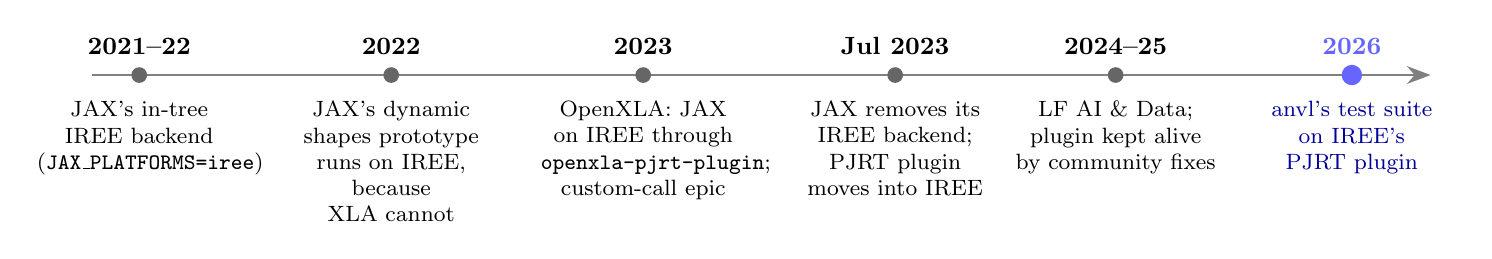
\begin{tikzpicture}[
  every node/.style={font=\small},
  tick/.style={circle, fill=black!60, inner sep=2pt},
  ours/.style={circle, fill=blue!60, inner sep=2.6pt},
  year/.style={font=\small\bfseries, above=4pt},
  event/.style={font=\footnotesize, below=6pt, align=center, text width=2.6cm}
]
  \draw[-{Stealth[length=3mm]}, thick, draw=black!50] (-0.6, 0) -- (16.4, 0);

  \node[tick] (a) at (0, 0) {};
  \node[year] at (a) {2021--22};
  \node[event] at (a) {JAX's in-tree IREE backend (\texttt{JAX\_PLATFORMS=iree})};

  \node[tick] (b) at (3.2, 0) {};
  \node[year] at (b) {2022};
  \node[event] at (b) {JAX's dynamic shapes prototype runs on IREE, because XLA cannot};

  \node[tick] (c) at (6.4, 0) {};
  \node[year] at (c) {2023};
  \node[event] at (c) {OpenXLA: JAX on IREE through \texttt{openxla-pjrt-plugin}; custom-call epic};

  \node[tick] (d) at (9.6, 0) {};
  \node[year] at (d) {Jul 2023};
  \node[event] at (d) {JAX removes its IREE backend; PJRT plugin moves into IREE};

  \node[tick] (e) at (12.4, 0) {};
  \node[year] at (e) {2024--25};
  \node[event] at (e) {LF AI \& Data; plugin kept alive by community fixes};

  \node[ours] (f) at (15.4, 0) {};
  \node[year, text=blue!60] at (f) {2026};
  \node[event, text=blue!60!black] at (f) {anvl's test suite on IREE's PJRT plugin};
\end{tikzpicture}
\end{document}
